\chapter{DevOps}
Nello sviluppo del software sia ha una collaborazione tra 2 team:
\begin{itemize}
      \item \textbf{Development}: si occupa di sviluppare l'applicazione e
            testarla.
      \item \textbf{Operation}: si occupa di pacchettizzarla e successivamente
            rilasciarla.
\end{itemize}
Il problema di questa organizzazione è che spesso i due team non comunicano, di
conseguenza si rende più costoso e lento il processo di rilascio.

Negli ultimi tempi si è sviluppato un altro metodo, chiamato \textbf{DevOps},
dove anche la parte di \textbf{operation} deve essere agile: il rilascio in
produzione e il deployment devono essere agili quanto lo sviluppo.

Si utilizzerà \textbf{DevOps} (\ref{fig:devops}) che permette di collegare ed
automatizzare lo sviluppo, il testing, la pacchettizzazione e il rilascio del
software. In questo modo si risolvono tutti i problemi introdotti precedentemente,
velocizzando tutto il processo di produzione del software.
\begin{figure}[!ht]
      \centering
      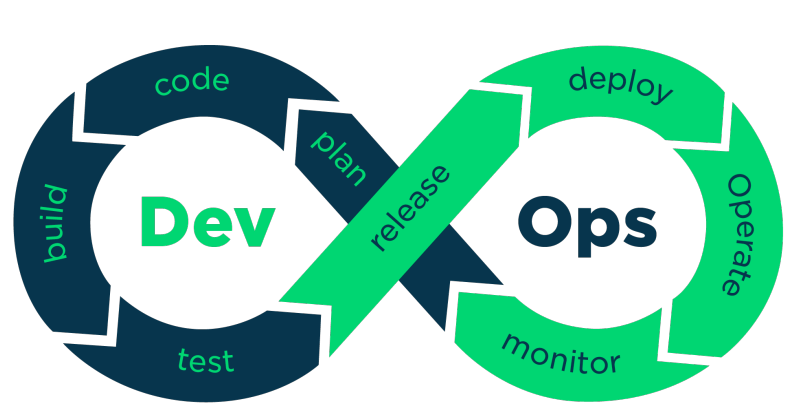
\includegraphics[width=0.5\textwidth]{img/devops/devops.png}
      \caption{Rappresentazione del lifecycle di DevOps}
      \label{fig:devops}
\end{figure}
DevOps promuove la collaborazione tra di due team al fine di ottenere una sorta
di team unico che curi sia sviluppo, sia operation. DevOps include quindi diversi
processi che vengono automatizzati:
\begin{itemize}
      \item Continuous Development
      \item Continuous Integration
      \item Continuous Testing
      \item Continuous Deployment
      \item Continuous Monitoring
\end{itemize}
L'automatizzazione è possibile grazie all'utilizzo della virtualizzazione
dell'hardware mediante macchine virtuali o container.

Con DevOps il feedback arriva anche dal software inoltre il focus viene
spostato sui processi automatici. Nel DevOps si introducono nuovi ruoli:
\begin{itemize}
      \item \textbf{DevOps Evangelist}: simile allo scrum master, supervisiona
            l'intero processo di DevOps.
      \item \textbf{Automation expert}: dedicato a curare gli aspetti di
            automatismo.
      \item \textbf{Security Engineer}
      \item \textbf{Software Developer}: nonché Tester.
      \item \textbf{Quality Assurance}: verifica la qualità del prodotto
            rispetto ai requisiti.
      \item \textbf{Code Release Manager}: si occupa sull'infrastruttura e
            sul deploy della release.
\end{itemize}
DevOps si basa su sei principi base:
\begin{enumerate}
      \item \textbf{Customer-Centric Action}: il committente è al centro dell'azione.
      \item \textbf{End-To-End Responsibility}: il team gestisce interamente
            il prodotto, avendone responsabilità totale.
      \item \textbf{Continuous Improvement}: cercare continuamente di migliorare
            senza sprechi il prodotto finale e i servizi.
      \item \textbf{Automate everything}: cercare di automatizzare l'intera
            infrastruttura di processo, dalle attività di testing e integrazione
            fino ad arrivare alla costruzione della release e del deployment.
      \item \textbf{Work as one team}: unificare tutti gli aspetti sotto un
            unico team o comunque con due team che collaborano fortemente come
            se fossero uno.
      \item \textbf{Monitor and test everything}: testare e monitorare
            costantemente il prodotto.
\end{enumerate}
Il quarto e il sesto punto sono i due punti tecnici principali.
\section{Build, Test e Release}
Bisogna pensare a questi step in ottica di automatismo vicina al DevOps.
Innanzitutto bisogna introdurre i sistemi di version control (Git) un sistema di
version control distribuito, dove ogni utente ha una copia della repository
(con la storia dei cambiamenti), con la quale interagisce tramite commit e update.
Esiste poi una repository lato server per permettere di condividere i vari
cambiamenti tramite sincronizzazione. Nello sviluppo multi-branch si segue il
seguente standard:
\begin{itemize}
      \item Master: branch utilizzato per salvare tutte le versioni di production,
            quindi quando si fa il push allora si eseguono tutte le operazioni
            automatiche di DevOps.
      \item HotFix: branch utile per eventuali Fix veloci della production.
      \item Release: branch su cui fare il push prima di mandare su master per
            il deploy.
      \item Develop: branch effettivo su cui verranno fatti i merge delle
            varie features.
      \item 1 branch per ogni feature da sviluppare.
\end{itemize}
\begin{figure}[!ht]
      \centering
      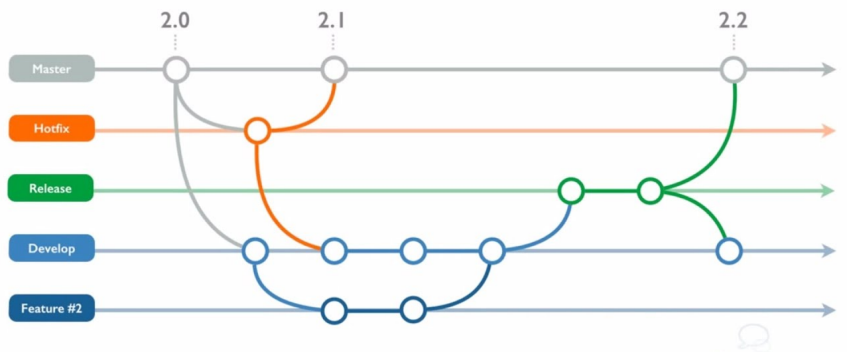
\includegraphics[width=0.5\textwidth]{img/devops/git.png}
      \caption{Struttura ideale di un repository git}
      \label{fig:git}
\end{figure}
Lo sviluppo su multi-branch si collega alle operazioni di verifica che possono
essere attivate automaticamente a seconda dell'evoluzione del codice su ogni branch.
Avendo ogni branch una precisa semantica possiamo definire precise attività di
verifica, corrispondenti a pipelines precise, solitamente innescate da un push di
codice su un certo branch, in modo sia automatico che manuale.
Le pipeline vengono attivate in fase di test di un componente, in fase di creazione
di un sottosistema, di assembramento di un sistema intero o di deployment in
produzione. In queste fase di DevoOps si possono riconoscere le seguenti sottofasi:
\begin{enumerate}
      \item \textbf{Component phase}
      \item \textbf{Subsystem phase}
      \item \textbf{System phase}
      \item \textbf{Production phase}
\end{enumerate}
Spesso le pipelines sono usate come \textbf{quality gates} per valutare se un push
può essere accettato in un certo branch. Una pipeline può essere anche regolata
temporalmente, in modo che avvenga solo ad un certo momento della giornata.
\subsection{Component phase e Subsystem phase}
Dove il focus è sulla più piccola unità testabile che viene aggiornata che non
può essere eseguita senza l'intero sistema. In tal caso si può fare:
\begin{itemize}
      \item Code review
      \item Unit testing
      \item Static code analysis
\end{itemize}
Un cambiamento può anche essere testato nell'ambito del sottosistema di cui fa
parte, in tal caso si hanno anche check di prestazioni e sicurezza. Il servizio
però potrebbe essere da testare in isolamento rispetto ad altri servizi, usando
quindi dei mocks o degli stubs, ovvero creando degli alter ego dei servizi mancanti
in modo che il servizio da testare possa funzionare.
\subsection{System phase}
In questo caso si testa l'intero sistema che viene rilasciato in ambiente di test.
Si hanno:
\begin{itemize}
      \item \textbf{Test funzionali}: test su ogni singola funzione (unit e integration).
      \item \textbf{Test di performance}: controlla le performance della release.
      \item \textbf{Security checks}: controllo automatico delle falle su metodi conosciuti
            (penetration test).
\end{itemize}
Tutti test che richiedono l'interezza del sistema sono spesso molto dispendiosi
e quindi bisogna regolare la frequenza di tali test in molti casi.
\subsection{Production phase}
Questa fase è legata alla necessità di creare gli artefatti che andranno
direttamente “sul campo”, ovvero il deployment in produzione. In tale fase potrebbe
essere necessario creare container o macchine virtuali. Si hanno dei check molto
veloci sugli artefatti finali, dando per assodato che la qualità del codice sia
già stata testata. Si hanno quindi strategie anche di deployment incrementale, per
cui esistono più versioni del software contemporaneamente con diversa accessibilità
per gli utenti finali. In tal caso si usano anche vari tool di monitor. Si hanno
anche eventualmente tecniche di zero downtime.

Fasi diverse corrispondono a branch diversi
\section{Deploy, Operate e Monitor}
Si studia l'evoluzione automatica del software da una versione all'altra in
produzione. Avanzare di versione in modo naive e istantaneo è troppo rischioso e
quindi spesso non attuabile. Si ha quindi un insieme di tecniche per la version
migration che si basano sull'evoluzione incrementale.

Tali tecniche si distinguono in base alla dimensione su cui sono incrementati:
\begin{itemize}
      \item \textbf{Incremental with reference to users}: Dark launching, Canary
            releases (and User Experimentation), ovvero legata agli utenti esposti
            alla nuova release.
      \item \textbf{Incremental with reference to requests}: Gradual upgrades/rollout,
            ovvero legata alle richieste per la nuova release.
      \item \textbf{Incremental with reference to components/replicas}: Rolling
            upgrade, incentrata sulle componenti che vengono aggiornate.
      \item \textbf{Non-incremental with backups}: Green/blue deployment,
            Rainbow deployment, non incrementali ma che offrono comunque un backup
            di sicurezza.
\end{itemize}
Tali schemi possono essere usati in un contesto DevOps. Per studiare la prima
tipologia (Incremental with reference to users) abbiamo:
\begin{itemize}
      \item \textbf{Dark launching}: in tale schema l'update è esposto solo ad una
            parte della popolazione, per la quale viene effettuato il deployment
            per studiare gli effetti ed eventuali modifiche e migliorie al
            software che, infine, verrà deployato per il resto della popolazione
            in modo comunque incrementale fino a che l'intera popolazione godrà
            della feature.
      \item \textbf{Canary releases}: come il Dark launching ma applicato alla
            migrazione del backend.
\end{itemize}
Tali schemi spesso sono usati di pari passo per le varie sezioni del software,
nonché possono essere usati in modo incrementale.

Collegato a questi schemi si ha l'approccio basato sull'\textbf{user experimentation},
che non è un reale schema di gestione dell'evoluzione del software ma è comunque
correlato agli schemi sopra descritti. In questo approccio si studiano diverse
varianti del sistema e il loro impatto esponendole agli utenti, cercando di capire
per l'utente cosa sia meglio e come. Si hanno quindi più release diverse, per
parti di popolazione comparabili, tra le quali si sceglierà la migliore.

Per la seconda tipologia (Incremental with reference to requests) si ha una
divisione a seconda delle richieste fatte dagli utenti, detto \textbf{gradual
      rollout}. Si ha quindi un load balancer che permette la coesistenza di due
versioni, una nuova e una vecchia, dello stesso servizio. In modo graduale,
partendo da pochissime, si passano le richieste alla versione nuova per poter
studiare e testare la nuova versione. Alla fine tutto il traffico sarà diretto
verso la nuova versione, mentre la vecchia verrà dismessa.

Per la terza tipologia (Incremental with reference to components/replicas),
si ha lo schema del \textbf{rolling upgrade}, dove l'upgrade non riguarda un
singolo upgrade ma tanti componenti di un sistema distribuito, verificando efficacia
di ogni singolo update tramite il continuous monitoring prima di effettuare l'upgrade
di un'altra componente. La stessa idea si applica anche a diverse versioni dello
stesso prodotto, aggiornandone una prima e poi le altre progressivamente. In
sostanza si aggiorna un container/VM alla volta.

Per la quarta tipologia (Non-incremental with backups) si ha il
\textbf{blue/green deployment}, dove vengono isolate due copie della stessa
infrastruttura, dove una ospita la versione nuove l'altra la vecchia. Un router
indirizza le richieste degli utenti verso le due unità e quella che ospita la
nuova versione subirà le solite operazioni di test che, se superate, porteranno
il router a direzionare verso quella unità, ignorando la vecchia. Se ci sono problemi
si fa rollback alla vecchia unità che rimane come backup. Questo schema può essere
generalizzato nel \textbf{rainbow deployment} dove il momento di coesistenza tra le due
versioni viene prolungato al fine che vecchie richieste che richiedono una lunga
elaborazione vengano elaborate dall'unità vecchia mentre le nuove dall'unità nuova.

In ogni caso le applicazioni devono essere costruite per supportare tutti questi
schemi di deployment perché bisogna specificare come gestire le richieste stateful
e i dati persistenti.
\subsection{Deployable units}
Il caso più tipico in merito alle unità dove fare deployment è il mondo del cloud
con unità virtualizzate e virtual machine (VM), dove magari ogni servizio vive in
una diversa VM. Si hanno diversi casi in merito a questo tipo di deployment:
\begin{itemize}
      \item \textbf{Cloud basato su VMs}: si ha un'infrastruttura gestita
            dal cloud provider che gestisce l'hardware e l'hypervisor. Ogni VM,
            che sono le nostre unità di deployment, ha un sistema operativo
            arbitrario che lavora con l'hardware mostrato dall'hypervisor. Ogni
            VM avrà una o più applicazioni e fare deployment porterà all'update
            di una o più VM. In alcuni casi si fa deployment di intere VM e in
            altri si modifica il software di una VM già in esecuzione. L'ambiente
            cloud solitamente è multi-tenant, ovvero su una piattaforma unica di
            un provider si hanno più VM di diverse organizzazioni.
            Una VM è grossa in quanto contiene un sistema operativo intero e la
            loro gestione può quindi essere difficoltosa.
      \item \textbf{Cloud basato su containers}: risolvono il problema della
            grandezza delle VM. In questo caso lo schema è il medesimo ma si ha
            un container engine al posto dell'hypervisor e ogni container non
            contiene l'intero sistema operativo ma solo il minimo necessario al
            funzionamento dell'applicazione. In questo caso lo schema di update
            spesso consiste nel distruggere e ricreare i singoli containers.
            Anche qui si ha un contesto multi-tenant.
      \item \textbf{Bare metal}: dove i provider offrono direttamente risorse
            hardware, guadagnando prestazioni ma aumentano anche i costi economici
            che vengono comunque gestite dal cloud provider. Non si ha
            virtualizzazione ma accesso diretto alle risorse su cui fare
            deployment. Questa è una soluzione tipicamente single-tenant.
      \item \textbf{Server dedicati}: un metodo ormai superato con difficoltà
            causate dall'uso di script, shell e connessione ftp completamente 
            autogestiti dall'organizzazione e non da un provider.
      \item \textbf{Non service software}: il software si rilascia su piattaforme
            di distribuzione, abbandonando l'idea della gestione del software
            come servizio.
\end{itemize}
Il deployment “stile cloud” non è comunque l'unico possibile.
\subsection{Monitor}
In ambiente cloud ci sono tante soluzioni per il monitoring, ad esempio lo stack
di ELK, formato da:
\begin{itemize}
      \item Elasticsearch
      \item Logstash
      \item Kibana
\end{itemize}
I dati, ad esempio log o metriche d'uso hardware, vengono raccolti e passano da
Logstash, finendo in un database, per la memorizzazione di time series (serie
temporali) di dati (questo in primis per le metriche d'uso che per i log), gestito
da Elasticsearch e venendo visualizzati da una dashboard grafica, gestita da
Kibana. Si ha quindi un ambiente di continuous monitoring.
\subsection{DevOps tools}
Ogni step del DevOps è gestito tramite moderne tecnologie e tools, con varie
alternative per ogni fase (per questo servono figure esperte per ogni step).
